% easy/easy.tex
% mainfile: ../perfbook.tex
% SPDX-License-Identifier: CC-BY-SA-3.0

\QuickQuizChapter{chp:Ease of Use}{Ease of Use}{qqzeasy}
%
\Epigraph{Creating a perfect API is like committing the perfect crime.
	  There are at least fifty things that can go wrong, and if you are
	  a genius, you might be able to anticipate twenty-five of them.}
	 {\emph{With apologies to any Kathleen Turner fans who might
	  still be alive.}}

\section{What is Easy?}
\label{sec:easy:What is Easy?}
%
\epigraph{When someone says ``I want a programming language in which I
	  need only say what I wish done,'' give them a lollipop.}
	 {\emph{Alan J.~ Perlis, updated}}
% http://www.cs.yale.edu/homes/perlis-alan/quotes.html

사용 편의성 요구사항을 들여다보고자 한다면, 리눅스 커널 RCU 의 사용 편의성
버그가 RCU 사용을 통해 이용될 수 있는 리눅스 커널 보안 버그를 초래했음을 고려해
주십시오.

불행히도, ``편하다'' 는 상대적인 용어입니다.
예를 들어, 많은 사람들이 15 시간의 비행기 여행을 약간의 고난으로
여깁니다---이동의 대안적인 모드, 특히 수영을 생각하하는 걸 멈추지 않는다면.
이는 사용하기 편한 API 를 만드는 것은 여러분이 여러분의 의도된 사용자들이
사용하기에 무엇이 편한지를 충분히 이해할 것을 요구함을 의미합니다.
여러분에게의 편의를 위해 무얼 하고 뭘 하지 않아야 할까요.

다음 질문이 그 요지를 보입니다:
``오늘날 살아있는 인류 가운데 무작위로 골라진 사람에게 어떤 변화가 그 사람의
인생을 개선시킬까?''

\iffalse

If you are tempted to look down on ease-of-use requirements, please
consider that an ease-of-use bug in Linux-kernel RCU resulted in an
exploitable Linux-kernel security bug in a use of
RCU~\cite{McKenney:2019:CRS:3319647.3325836}.
It is therefore clearly important that even in-kernel APIs be easy to use.

Unfortunately, ``easy'' is a relative term.
For example, many people would consider a 15-hour airplane flight to be
a bit of an ordeal---unless they stopped to consider alternative modes
of transportation, especially swimming.
This means that creating an easy-to-use API requires that you understand
your intended users well enough to know what is easy for them.
Which might or might not have anything to do with what is easy for you.

The following question illustrates this point: ``Given a randomly chosen
person among everyone alive today, what one change would
improve that person's life?''

\fi

모두의 삶을 도울 것이 보장된 하나의 변화는 존재하지 않습니다.
어쨌건, 엄청나게 다양한 사람이 존재하며, 그들의 필요한 것, 원하는 것, 소망,
그리고 포부도 모두 다양합니다.
기아로 굶주리는 사람은 음식을 필요로 할테지만 병적으로 비만인 사람에게 추가적인
음식은 죽음을 앞당길 겁니다.
많은 젊은 사람들에게 열렬히 소망될 높은 단계의 즐거움은 어떤 사람에게는 심장
마비에서 회복되기에 치명적일 겁니다.
어떤 사람에게는 성공을 위해 치명적인 정보가 정보 과다로 고통받는 누군가에게는
문제가 될 수도 있을 겁니다.
요약하자면, 여러분이 아무것도 모르는 사람들을 돕고자 기획된 소프트웨어
프로젝트를 위해 일하고 있다면, 여러분은 그 사람들이 여러분의 프로젝트에 문제를
발견해도 놀라지 않아야 합니다.

여러분이 정말로 해당 사람들을 돕고자 한다면 추가된 기간, 거의 수년 동안을
그들과 가깝게 일하는 것 외에는 간단한 대안이 없습니다.
그러나, 여러분의 이상한 사용자들이 여러분의 소프트웨어에 행복해지는 경우를
증가시키기 위해 여러분이 할 수 있는 몇가지 간단한 것들이 있으며, 이 간단한
것들이 다음 섹션에서 다루어집니다.

\iffalse

There is no single change that would be guaranteed to help everyone's life.
After all, there is an extremely wide range of people, with a correspondingly
wide range of needs, wants, desires, and aspirations.
A starving person might need food, but additional food might well hasten
the death of a morbidly obese person.
The high level of excitement so fervently desired by many young people
might well be fatal to someone recovering from a heart attack.
Information critical to the success of one person might contribute to
the failure of someone suffering from information overload.
In short, if you are working on a software project that is intended to
help people you know nothing about, you should not be surprised when
those people find fault with your project.

If you really want to help a given group of people, there is simply no
substitute for working closely with them over an extended period of time,
as in years.
Nevertheless, there are some simple things that you can do to increase
the odds of your users being happy with your software, and some of these
things are covered in the next section.

\fi

\section{Rusty Scale for API Design}
\label{sec:easy:Rusty Scale for API Design}
%
\epigraph{Finding the appropriate measurement is thus not a mathematical
	  exercise.  It is a risk-taking judgment.}
	 {\emph{Peter Drucker}}
% http://billhennessy.com/simple-strategies/2015/09/09/i-wish-drucker-never-said-it
% Rusty is OK with this: July 19, 2006.

이 섹션은 Rusty Russell 의 2003년 Ottawa Linux 심포지엄 키노드의
일부~\cite[Slides~39--57]{RustyRussell2003OLSkeynote} 를 수정했습니다.
Rusty 의 요점은 목적은 단순히 사용하기 편한 API 를 만드는 게 아니라 API 를 잘못
사용하기 어렵게 해야 한다는 겁니다.
그 결과, Rusty 는 그의 ``Rusty Scale'' 을 이 오용하기 어렵기 속성의 중요도의
내림차순으로 제안합니다.

다음 리스트는 Rusty Scale 을 리눅스 커널에 맞춰 일반화 해보려는 시도입니다:

\iffalse

This section is adapted from portions of Rusty Russell's 2003 Ottawa Linux
Symposium keynote address~\cite[Slides~39--57]{RustyRussell2003OLSkeynote}.
Rusty's key point is that the goal should not be merely to make an API
easy to use, but rather to make the API hard to misuse.
To that end, Rusty proposed his ``Rusty Scale'' in decreasing order
of this important hard-to-misuse property.

The following list attempts to generalize the Rusty Scale beyond the
Linux kernel:

\fi

\begin{enumerate}
\item	잘못되기 불가능할 것.
	이는 모든 API 설계자드리 추구해야 하는 표준이지만 상상의
		\co{dwim()}\footnote{
		\co{dwim()} 함수는 ``do what I mean'' 으로 펼쳐지는
		축약어입니다.}
	커맨드만이 근접할 수 있었습니다.
\item	컴파일러나 링커가 여러분이 잘못을 저지르게 못하게 할 것.
\item	컴파일러나 링커는 여러분이 뭔가 잘못하면 경고할 것.
	\co{BUILD_BUG_ON()} 은 여러분의 사용자의 친구가 됩니다.
\item	가장 간단한 사용이 올바른 방법일 것.
\item	이름이 사용법을 설명하게 하기.
	하지만 이름은 양날의 검입니다.
	비록 \co{rcu_read_lock()} 이 코드를 reader-writer 락킹으로부터
	변환하고자 하는 누군가에겐 충분히 평범하지만, 레퍼런스 카운팅에서
	코드를 변환하는 사람에겐 어떤 경악을 금치 못하게 할수도 있을 겁니다.
\item	올바르게 하지 않으면 수행시간에 항상 고장나게 하기.
	\co{WARN_ON_ONCE()} 가 여러분의 사용자의 친구가 됩니다.

\iffalse

\item	It is impossible to get wrong.
	Although this is the standard to which all API designers should
	strive, only the mythical \co{dwim()}\footnote{
		The \co{dwim()} function is an acronym that expands to
		``do what I mean''.}
	command manages to come close.
\item	The compiler or linker won't let you get it wrong.
\item	The compiler or linker will warn you if you get it wrong.
	\co{BUILD_BUG_ON()} is your users' friend.
\item	The simplest use is the correct one.
\item	The name tells you how to use it.
	But names can be two-edged swords.
	Although \co{rcu_read_lock()} is plain enough for someone
	converting code from reader-writer locking, it might cause
	some consternation for someone converting code from
	reference counting.
\item	Do it right or it will always break at runtime.
	\co{WARN_ON_ONCE()} is your users' friend.

\fi

\item	일반적인 관습을 따르면 올바르게 되기.
	\co{malloc()} 라이브러리 함수가 좋은 예입니다.
	메모리 할당을 잘못하기는 쉽지만 수많은 프로젝트가 적어도 대부분의 경우
	이를 올바르게 관리합니다.
	\co{malloc()} 을 Valgrind~\cite{ValgrindHomePage} 와 함께 사용하는 것은
	\co{malloc()} 을 거의 ``올바르게 하지 않으면 수행시간에 항상 고장나게
	하기'' 지점까지 옮깁니다.
\item	문서를 읽으면 올바르게 사용할 수 있게 하기.
\item	구현을 읽으면 올바르게 사용할 수 있게 하기.
\item	올바른 메일링 리스트 기록을 읽으면 올바르게 사용할 수 있게 하기.
\item	올바른 메일링 리스트 기록을 읽으면 잘못 사용하게 하기.
\item	구현을 읽으면 잘못 사용하게 하기.
	\co{rcu_read_lock()} 의 최초 비 \co{CONFIG_PREEMPT}
	구현은~\cite{PaulEMcKenney2007PreemptibleRCU} 이 지점의 확장성에 대한
	악명 높은 예입니다.

\iffalse

\item	Follow common convention and you will get it right.
	The \co{malloc()} library function is a good example.
	Although it is easy to get memory allocation wrong, a
	great many projects do manage to get it right, at least most
	of the time.
	Using \co{malloc()} in conjunction with
	Valgrind~\cite{ValgrindHomePage} moves \co{malloc()}
	almost up to the ``do it right or it will always break at runtime''
	point on the scale.
\item	Read the documentation and you will get it right.
\item	Read the implementation and you will get it right.
\item	Read the right mailing-list archive and you will get it right.
\item	Read the right mailing-list archive and you will get it wrong.
\item	Read the implementation and you will get it wrong.
	The original non-\co{CONFIG_PREEMPT} implementation of
	\co{rcu_read_lock()}~\cite{PaulEMcKenney2007PreemptibleRCU}
	is an infamous example of this point on the scale.

\fi

\item	문서를 읽으면 잘못 사용하게 하기.
	예를 들어, DEC Alpha \co{wmb} 명령의 문서는~\cite{ALPHA2002} 많은
	개발자들로 하여금 이 명령이 실제보다 훨씬 강력한 메모리 순서 규칙을
	갖는 걸로 오해하게 만들었습니다.
	나중의 문서는 이 지점을 분명케
	했고~\cite{Compaq01,WilliamPugh2000Gharachorloo}, \co{wmb} 명령을
	``문서를 읽으면 올바르게 사용하게 하기'' 지점까지 올려놓았습니다.
\item	흔한 관례를 따르면 잘못 사용하게 하기.
	\co{printf()} 문은 이 지점의 한 예인데, 개발자들은 거의 항상
	\co{printf()} 의 반환 오류를 검사하지 않기 때문입니다.
\item	올바르게 사용하면 수행 시간에 고장나게 하기.
\item	이름이 그것을 어떻게 사용하면 안되는지 말하게 하기.

\iffalse

\item	Read the documentation and you will get it wrong.
	For example, the DEC Alpha \co{wmb} instruction's
	documentation~\cite{ALPHA2002} fooled a
	number of developers into thinking that this instruction
	had much stronger memory-order semantics than it actually does.
	Later documentation clarified this
	point~\cite{Compaq01,WilliamPugh2000Gharachorloo},
	moving the \co{wmb} instruction up to the
	``read the documentation and you will get it right'' point on
	the scale.
\item	Follow common convention and you will get it wrong.
	The \co{printf()} statement is an example of this point on the
	scale because
	developers almost always fail to check \co{printf()}'s error return.
\item	Do it right and it will break at runtime.
\item	The name tells you how not to use it.

\fi

\item	명백한 사용이 잘못되기.
	리눅스 커널의 \co{smp_mb()} 함수는 이 지점의 한 예입니다.
	많은 개발자들이 이 함수가 실제로 수행하는 것보다 훨씬 강한 순서 규칙을
	갖는다고 가정합니다.
	Chapter~\ref{chp:Advanced Synchronization: Memory Ordering} 가 이
	실수를 막기 위한 정보를 리눅스 커널 소스 트리의
	\path{Documentation} 과 \path{tools/memory-model} 디렉토리들처럼 담고
	있습니다.
\item	컴파일러나 링커가 여러분이 올바른 사용을 했을때 경고를 하기.
\item	컴파일러나 링커가 여러분이 올바른 사용을 할 수 없게 하기.
\item	올바르게 사용하기가 불가능하기.
	\co{gets()} 함수는 이 지점의 유명한 예입니다.
	사실, \co{gets()} 는 무조건적 버퍼 오버플로우 보안 구멍으로 가장 잘
	설명될 수도 있을 겁니다.

\iffalse

\item	The obvious use is wrong.
	The Linux kernel \co{smp_mb()} function is an example of
	this point on the scale.
	Many developers assume that this function has much
	stronger ordering semantics than it actually possesses.
	Chapter~\ref{chp:Advanced Synchronization: Memory Ordering} contains the
	information needed to avoid this mistake, as does the
	Linux-kernel source tree's \path{Documentation} and
	\path{tools/memory-model} directories.
\item	The compiler or linker will warn you if you get it right.
\item	The compiler or linker won't let you get it right.
\item	It is impossible to get right.
	The \co{gets()} function is a famous example of this point on
	the scale.
	In fact, \co{gets()} can perhaps best be described as
	an unconditional buffer-overflow security hole.

\fi

\end{enumerate}

\section{Shaving the Mandelbrot Set}
\label{sec:easy:Shaving the Mandelbrot Set}
%
\epigraph{Simplicity does not precede complexity, \\ but follows it.}
	 {\emph{Alan J.~Perlis}}

유용한 프로그램들의 집합은 깨끗하게 구분되는 선이 없다는 점에서 Mandelbrot 집합
(Figure~\ref{fig:easy:Mandelbrot Set}에 보여 있습니다) 을 닮았습니다---만약
그런 선이 있다면, 이 문제는 해결 가능할 겁니다.
그러나 우리는 실제 사람들이 사용할 수 있는 API 가 필요하지, 모든 잠재적 사용을
위해 박사 학위를 필요로 하는 API 를 필요로 하지 않습니다.
따라서, 우린 ``Mandelbrot set 을 깎아내어''\footnote{
	Josh Triplett 덕입니다.}
API 의 사용을 잠재적 사용의 완벽한 집합의 쉽게 설명될 수 있는 부분집합으로
제한해야 합니다.

\iffalse

The set of useful programs resembles the Mandelbrot set
(shown in Figure~\ref{fig:easy:Mandelbrot Set})
in that it does
not have a clear-cut smooth boundary---if it did, the halting problem
would be solvable.
But we need APIs that real people can use, not ones that require a
Ph.D. dissertation be completed for each and every potential use.
So, we ``shave the Mandelbrot set'',\footnote{
	Due to Josh Triplett.}
restricting the use of the
API to an easily described subset of the full set of potential uses.

\fi

\begin{figure}[tbp]
\centering
\resizebox{2.5in}{!}{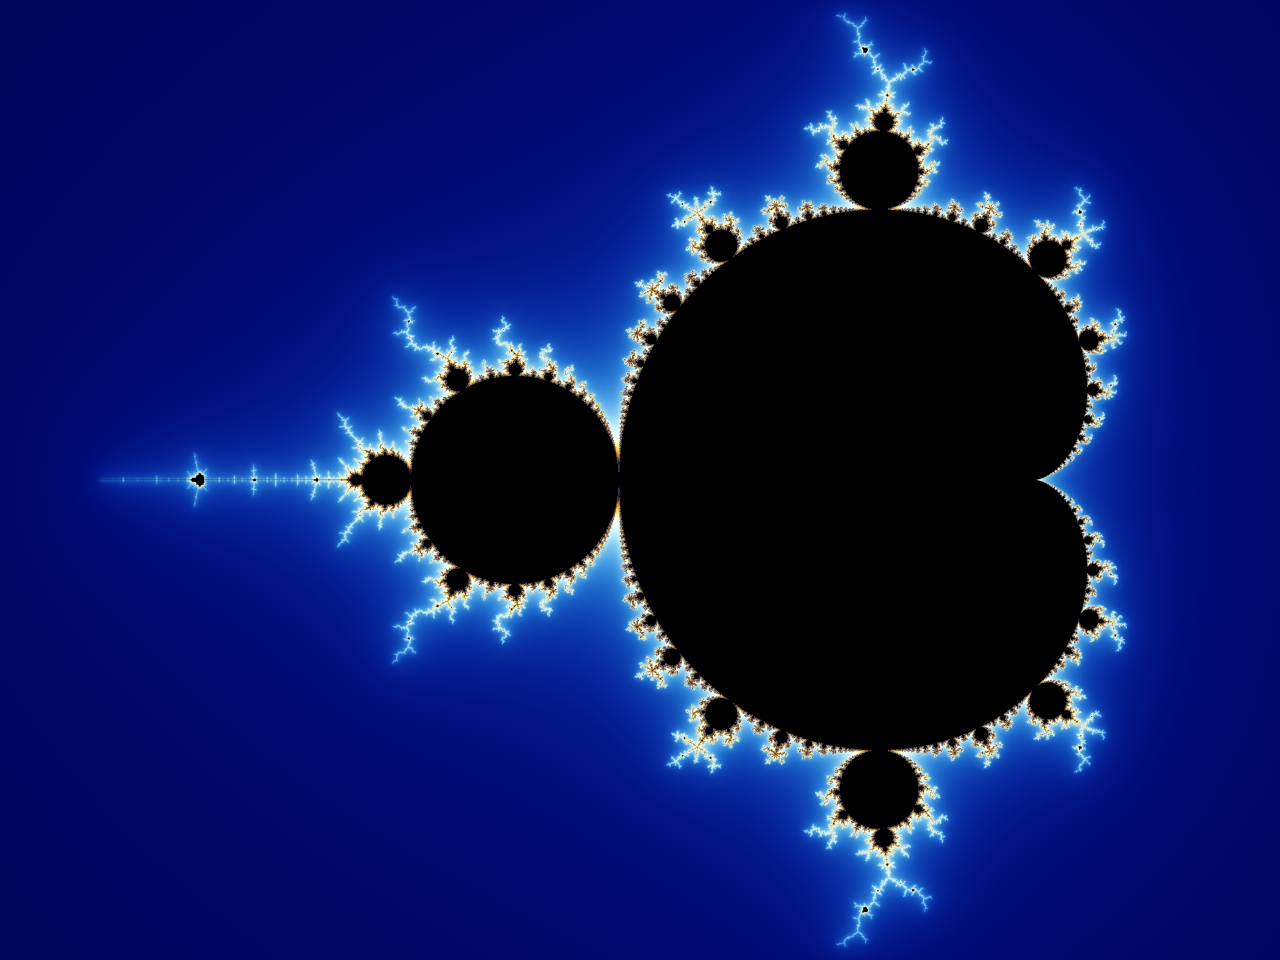
\includegraphics{easy/Mandel_zoom_00_mandelbrot_set}}
\caption{Mandelbrot Set (Courtesy of Wikipedia)}
\label{fig:easy:Mandelbrot Set}
\end{figure}

그런 깎아냄은 반생산적으로 보일 수 있습니다.
어쨌건, 어떤 알고리즘이 동작한다면, 왜 사용하지 않습니까?

왜 적어도 일부의 깎아냄은 반드시 필요한지 이해하기 위해, 데드락을 방지하지만
아마도 가능한 가장 나쁜 방법으로 그걸 하는 락킹 설계를 생각해 봅시다.
이 설계는 순환형 이중 링크드 리스트를 사용하는데, 이 리스트는 헤더 원소와 함께
시스템의 각 쓰레드를 위해 하나의 원소를 가집니다.
새로운 쓰레드가 생성될 때, 그 부모 쓰레드는 이 리스트에 새 원소를 삽입해야
하는데, 이는 어떤 종류의 동기화를 필요로 합니다.

\iffalse

Such shaving may seem counterproductive.
After all, if an algorithm works, why shouldn't it be used?

To see why at least some shaving is absolutely necessary, consider
a locking design that avoids deadlock, but in perhaps the worst possible way.
This design uses a circular doubly linked list, which contains one
element for each thread in the system along with a header element.
When a new thread is spawned, the parent thread must insert a new
element into this list, which requires some sort of synchronization.

\fi

이 리스트를 보호하기 위해 전역 락을 사용하는 방법이 있겠습니다.
그러나, 이는 쓰레드가 빈번히 생성되고 삭제된다면 병목이 될 수
있습니다.\footnote{
	운영체제에 대한 깊은 이해가 있는 분들이라면 부디 불신을 멈추십시오.
	불신을 멈출 수 없는 분들은 더 나은 예를 제공해주시면 좋겠습니다.}
또다른 방법은 해쉬 테이블을 사용하고 각 해쉬 버킷을 락킹하는 것입니다만 이는
리스트를 순서대로 수캐닝 하는 성능을 나쁘게 할 수 있습니다.

세번째 방법은 개별 리스트 원소를 락킹 하고 삽입 시에 그 앞과 뒤 원소들의 락도
잡게끔 하는 겁니다.
두 락이 모두 잡혀야 하므로, 우린 이걸 어느 순서로 잡을지 정해야 합니다.
두개의 관례적 방법은 이 락을 주소 순서대로 잡는 것, 또는 리스트에 나타나는
순서대로 잡아서 락킹 되는 두개의 원소 중 하나인 경우엔 그 헤더가 항상 먼저
잡히게 하는 겁니다.
그러나, 이 방법들 둘 다 특수한 검사와 분기를 필요로 합니다.

\iffalse

One way to protect the list is to use a global lock.
However, this might be a bottleneck if threads were being created and
deleted frequently.\footnote{
	Those of you with strong operating-system backgrounds, please
	suspend disbelief.
	Those unable to suspend disbelief are encouraged to provide
	better examples.}
Another approach would be to use a hash table and to lock the individual
hash buckets, but this can perform poorly when scanning the list in order.

A third approach is to lock the individual list elements, and to require
the locks for both the predecessor and successor to be held during the
insertion.
Since both locks must be acquired, we need to decide which order to
acquire them in.
Two conventional approaches would be to acquire the locks in address
order, or to acquire them in the order that they appear in the list,
so that the header is always acquired first when it is one of the two
elements being locked.
However, both of these methods require special checks and branches.

\fi

깎아내져야 하는 해결책은 리스트 순서대로 무조건적으로 락을 잡는 겁니다.
하지만 데드락은 어떡하죠?

데드락은 일어날 수 없습니다.

이를 보기 위해, 0에서 시작해 이 리스트의 마지막 원소에 (이 리스트가
순환형이므로, 헤더의 앞 원소가 됩니다) $N$ 까지 번호를 매겨봅시다.
비슷하게, 시스템의 쓰레드는 0 부터 $N-1$ 까지 번호를 매깁니다.
각 쓰레드가 어떤 연속적인 한쌍의 원소를 락킹하려 한다면, 그 쓰레드 중 하나는 두
락을 모두 획득할 수 있을 것이 보장됩니다.

\iffalse


The to-be-shaven solution is to unconditionally acquire the locks in
list order.
But what about deadlock?

Deadlock cannot occur.

To see this, number the elements in the list starting with zero for the
header up to $N$ for the last element in the list (the one preceding the
header, given that the list is circular).
Similarly, number the threads from zero to $N-1$.
If each thread attempts to lock some consecutive pair of elements,
at least one of the threads is guaranteed to be able to acquire both
locks.

\fi

왜일까요?

이 리스트의 전체에 닿기에는 쓰레드의 수가 충분치 않기 때문입니다.
쓰레드~0 이 원소~0 의 락을 잡으려 한다고 해봅시다.
블록되기 위해서는, 어떤 다른 쓰레드가 이미 원소~1 의 락을 잡았어야 하는데
쓰레드~1 이 그랬다고 해봅시다.
비슷하게, 쓰레드~1 이 블락되기 위해선 어떤 다른 쓰레드가 원소~2 의 락을
잡았어야 하며, 그런식으로 원소~$N-1$ 의 락을 잡고 있을 쓰레드~$N-1$ 까지
갑니다.
하지만 더이상의 쓰레드가 없으므로 쓰레드~$N-1$ 은 블록될 수 없습니다.
따라서, 데드락은 일어날 수 없습니다.

그러니 이 즐겁고 작은 알고리즘을 사용하지 않을 이유가 어디 있겠습니까?

사실 여러분이 \emph{정말로} 그걸 사용하고 싶어한다면 우린 여러분을 막을 수
없습니다.
그러나, 우리는 그런 코드가 우리가 신경쓰는 프로젝트에 포함되는 걸 반대할 수
\emph{있습니다}.

그러나, 이 알고리즘을 사용하기 전에, 다음 Quick Quiz 를 생각해 보세요.

\iffalse

Why?

Because there are not enough threads to reach all the way around the list.
Suppose thread~0 acquires element~0's lock.
To be blocked, some other thread must have already acquired element~1's
lock, so let us assume that thread~1 has done so.
Similarly, for thread~1 to be blocked, some other thread must have acquired
element~2's lock, and so on, up through thread~$N-1$, who acquires
element~$N-1$'s lock.
For thread~$N-1$ to be blocked, some other thread must have acquired
element~$N$'s lock.
But there are no more threads, and so thread~$N-1$ cannot be blocked.
Therefore, deadlock cannot occur.

So why should we prohibit use of this delightful little algorithm?

The fact is that if you \emph{really} want to use it, we cannot stop you.
We \emph{can}, however, recommend against such code being included
in any project that we care about.

But, before you use this algorithm, please think through the following
Quick Quiz.

\fi

\QuickQuiz{
	원소의 삭제에도 비슷한 알고리즘을 사용할 수 있나요?

	\iffalse

	Can a similar algorithm be used when deleting elements?

	\fi

}\QuickQuizAnswer{
	그렇습니다.
	그러나, 각 쓰레드는 가운데의 원소를 제거하기 위해 세개의 연속된 원소의
	락을 잡아야 하므로, $N$ 개 쓰레드가 있다면, 데드락을 막기 위해 그
	리스트에는 $N+1$ 개가 아니라 $2N+1$ 개 원소가 있어야 합니다.

	\iffalse

	Yes.
	However, since each thread must hold the locks of three
	consecutive elements to delete the middle one, if there
	are $N$ threads, there must be $2N+1$ elements (rather than
	just $N+1$) in order to avoid deadlock.

	\fi

}\QuickQuizEnd

여기서의 중요한 사실은 이 알고리즘은 극단적으로 특수화 되었으며 (특정한 크기의
리스트에서만 동작합니다), 잘못되기도 쉽다는 겁니다.
리스트에 노드를 추가하는데 사고로 실패하는 모든 버그는 데드락을 초래할 수
있습니다.
실제로, 노드를 약간 늦게 추가하는 것 만으로도 쓰레드의 수를 늘리는 게 그럴 수
있듯 데드락을 초래할 수 있습니다.

또한, 앞에서 설명된 다른 알고리즘은 ``좋고 충분합니다''.
예를 들어, 주소 순서로 락을 획득하는 건 충분히 간단하고 빠르며, 모든 크기의
리스트의 사용을 허용합니다.
다만 빈 리스트와 하나의 원소만 포함하는 리스트의 특수 경우에 주의하세요!

\iffalse

The fact is that this algorithm is extremely specialized (it only works
on certain sized lists), and also quite fragile.
Any bug that accidentally failed to add a node to the list could result
in deadlock.
In fact, simply adding the node a bit too late could result in deadlock,
as could increasing the number of threads.

In addition, the other algorithms described above are ``good and sufficient''.
For example, simply acquiring the locks in address order is fairly simple
and quick, while allowing the use of lists of any size.
Just be careful of the special cases presented by empty lists and lists
containing only one element!

\fi

\QuickQuiz{
	와우!
	도대체 무엇이 누군가로 하여금 이것 만큼 깎아낼 가치가 있는 알고리즘을
	생각해내게 할까요???

	\iffalse

	Yetch!
	What ever possessed someone to come up with an algorithm
	that deserves to be shaved as much as this one does???

	\fi

}\QuickQuizAnswer{
	그건 Paul 일 겁니다.

	그는 다섯명의 철학자가 참석하는 이상한 스파게티 저녁식사를 포함하는
	\emph{식사하는 철학자들의 문제} 를 생각하고 있었습니다.
	테이블에 다섯개의 쟁반에 다섯개의 포크만이 있다는 점으로 보아, 그리고
	각 철학자는 식사를 위해 한번에 두개의 포크를 필요로 한다는 점으로 보아,
	누군가는 데드락을 회피하는 포크 할당 알고리즘을 생각해낼 겁니다.
	Paul 의 답은 ``윽!  그냥 포크 다섯개를 더 줘!'' 였습니다.

	이것 자체로는 괜찮았습니다만, Paul 은 이 동일한 해결책을 순환 링크드
	리스트에 적용했습니다.

	이것 역시 크게 나쁘지 않았습니다만 그는 누군가에게 이를 이야기 해야만
	했습니다!

	\iffalse

	That would be Paul.

	He was considering the \emph{Dining Philosopher's Problem}, which
	involves a rather unsanitary spaghetti dinner attended by
	five philosophers.
	Given that there are five plates and but five forks on the table, and
	given that each philosopher requires two forks at a time to eat,
	one is supposed to come up with a fork-allocation algorithm that
	avoids deadlock.
	Paul's response was ``Sheesh!  Just get five more forks!''

	This in itself was OK, but Paul then applied this same solution to
	circular linked lists.

	This would not have been so bad either, but he had to go and tell
	someone about it!

	\fi

}\QuickQuizEnd

\begin{figure}[tbp]
\centering
\resizebox{2.5in}{!}{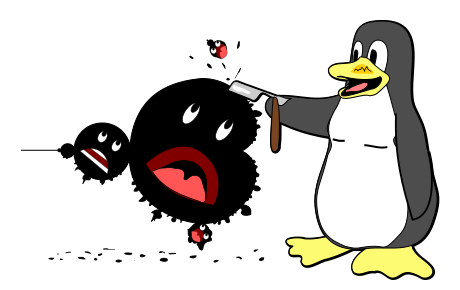
\includegraphics{cartoons/r-2014-shaving-the-mandelbrot}}
\caption{Shaving the Mandelbrot Set}
\ContributedBy{Figure}{fig:easy:Shaving the Mandelbrot Set}{Melissa Broussard}
\end{figure}

요약하자면, 우린 어떤 알고리즘을 그게 동작한다는 이유만으로 사용하지 않습니다.
우린 그대신 그걸 배울 가치가 충분할 정도로 충분히 유용한 알고리즘들만
사용합니다.
그 알고리즘이 더 어렵고 복잡하다면, 그것은 더 일반적으로 유용해서 그걸 배우고
그것의 버그를 고치는 고통이 가치있게 해야 합니다.

\iffalse

In summary, we do not use algorithms simply because they happen to work.
We instead restrict ourselves to algorithms that are useful enough to
make it worthwhile learning about them.
The more difficult and complex the algorithm, the more generally useful
it must be in order for the pain of learning it and fixing its bugs to
be worthwhile.

\fi

\QuickQuiz{
	이 규칙에 대한 예외를 하나 주세요.

	\iffalse

	Give an exception to this rule.

	\fi

}\QuickQuizAnswer{
	이에 대한 예외 하나는 특정 상황에 동작하는 유일한 것으로 알려진 어렵고
	복잡한 알고리즘을 겁니다.
	또다른 예외는 해당 상황에서 동작하는 것으로 알려진 것들 중 가장 간단한,
	그러나 여전히 어렵고 복잡한 알고리즘을 겁니다.
	그러나, 이 경우에도, 더 간단한 알고리즘을 찾기 위해 약간의 시간을
	사용하는게 매우 가치있을 겁니다!
	어쨌건, 어떤 작업을 위한 첫번째 알고리즘을 발명해 냈다면, 더 간단한
	것을 발명하는게 그렇게 어렵지만은 않을 겁니다.

	\iffalse

	One exception would be a difficult and complex algorithm that
	was the only one known to work in a given situation.
	Another exception would be a difficult and complex algorithm
	that was nonetheless the simplest of the set known to work in
	a given situation.
	However, even in these cases, it may be very worthwhile to spend
	a little time trying to come up with a simpler algorithm!
	After all, if you managed to invent the first algorithm
	to do some task, it shouldn't be that hard to go on to
	invent a simpler one.

	\fi

}\QuickQuizEnd

예외들을 제외하고도, 우린
Figure~\ref{fig:easy:Shaving the Mandelbrot Set} 에 보인 것처럼 우리의
프로그램이 유지가능하게 지속되게끔 소프트웨어 ``Mandelbrot set'' 을 깎아내기를
계속해야 합니다.

\iffalse

Exceptions aside, we must continue to shave the software ``Mandelbrot
set'' so that our programs remain maintainable, as shown in
Figure~\ref{fig:easy:Shaving the Mandelbrot Set}.

\fi

\QuickQuizAnswersChp{qqzeasy}
